\documentclass[conference]{IEEEtran}
\IEEEoverridecommandlockouts

\usepackage{cite}
\usepackage{amsmath,amssymb,amsfonts}
\usepackage{graphicx}
\usepackage{textcomp}
\usepackage{xcolor}
\usepackage[utf8]{inputenc}
\usepackage[spanish]{babel}
\usepackage{hyperref}
\usepackage{booktabs}
\usepackage{tikz}
\usetikzlibrary{arrows.meta,positioning,shapes.geometric,calc,fit,backgrounds}

\graphicspath{{img/}}

\def\BibTeX{{\rm B\kern-.05em{\sc i\kern-.025em b}\kern-.08em
    T\kern-.1667em\lower.7ex\hbox{E}\kern-.125emX}}

% --- estilos de diagramas de estados / bloques ---
\tikzset{
  state/.style={rectangle, rounded corners=3pt, draw=black!70, thick,
    fill=blue!6, align=center, minimum height=8mm, minimum width=15mm,
    font=\scriptsize\sffamily, inner sep=3pt},
  term/.style={rectangle, rounded corners=3pt, draw=black!70, thick,
    fill=green!10, align=center, minimum height=8mm, font=\scriptsize\sffamily, inner sep=3pt},
  node2/.style={rectangle, draw=black!60, thick, fill=orange!8, align=center,
    font=\scriptsize\sffamily, minimum height=7mm, inner sep=3pt},
  topic/.style={font=\tiny\ttfamily, text=black!55},
  tr/.style={-{Stealth[length=2mm]}, draw=black!70, font=\tiny\sffamily},
}

\begin{document}

\title{Localización y Mapeo Simultáneos con Landmarks Visuales, Navegación Autónoma y Exploración Informativa en un TurtleBot4:\\ Memoria Técnica del Trabajo Práctico Final}

\author{\IEEEauthorblockN{Tomás Benavidez Esposito}
\IEEEauthorblockA{\textit{Ingeniería en Inteligencia Artificial} \\
\textit{Universidad de San Andrés}\\
Buenos Aires, Argentina \\
tbenavidez@udesa.edu.ar}
\and
\IEEEauthorblockN{Naomi Couriel}
\IEEEauthorblockA{\textit{Ingeniería en Inteligencia Artificial} \\
\textit{Universidad de San Andrés}\\
Buenos Aires, Argentina \\
ncouriel@udesa.edu.ar}
}

\maketitle

\begin{abstract}
Presentamos la memoria técnica de un sistema robótico autónomo de localización y mapeo simultáneos (SLAM), navegación y exploración activa, desarrollado sobre la plataforma TurtleBot4 y ROS~2 Humble. El trabajo se estructura en tres etapas acopladas. En la \textbf{Parte~A} implementamos un \emph{Graph SLAM} sobre datos reales pregrabados (RosBag), fusionando el modelo de odometría por deltas con avistajes de marcadores \emph{ArUco} detectados por la cámara OAK-D; una primera pasada optimiza el grafo de poses con cierre de lazo y una segunda pasada proyecta el LIDAR sobre la trayectoria corregida para obtener una grilla de ocupación métrica. En la \textbf{Parte~B} desarrollamos la navegación autónoma (Sistema~3: grilla + landmarks de cámara) sobre Gazebo, integrando un filtro de partículas (MCL) que fusiona un modelo de haz láser con observaciones de un sensor virtual de landmarks con oclusión, un planificador global A$^\star$ con inflado y márgenes de seguridad, un seguidor \emph{pure-pursuit} y una máquina de estados que gobierna el ciclo completo, incluyendo detección y evasión de obstáculos no mapeados. En la \textbf{Parte~C} extendemos el sistema con una capa de misión de exploración informativa guiada por una función de utilidad y un módulo de percepción que detecta conos rojos por segmentación en HSV con validación geométrica y temporal, reproyectando la detección al planificador para respetar los muros reales. Reportamos los resultados cuantitativos obtenidos en simulación y sobre los RosBags del TurtleBot4 --- error de seguimiento del MCL de $0.02$--$0.18$~m y evasión sin colisión --- y documentamos las decisiones de diseño que hicieron converger cada subsistema. La validación sobre el robot físico (Parte~C) queda pendiente de la ventana de laboratorio y se detalla como trabajo a completar.
\end{abstract}

\begin{IEEEkeywords}
SLAM, Graph SLAM, ArUco, Monte Carlo Localization, filtro de partículas, navegación autónoma, A$^\star$, máquina de estados, exploración informativa, ROS~2, TurtleBot4.
\end{IEEEkeywords}

\section{Introducción}

La localización y el mapeo simultáneos (SLAM) constituyen uno de los problemas fundamentales de la robótica móvil: un robot que se desplaza por un entorno desconocido debe, al mismo tiempo, construir un mapa del entorno y estimar su propia posición dentro de él, empleando únicamente sensores inexactos y un modelo de movimiento afectado por ruido. Este trabajo práctico final integra los principales enfoques probabilísticos estudiados a lo largo de la materia \emph{Principios de la Robótica Autónoma} en un sistema completo que abarca desde la estimación de estado hasta la actuación autónoma.

El sistema se desarrolla en tres etapas encadenadas, en las que cada una consume el producto de la anterior:

\begin{itemize}
    \item \textbf{Parte~A --- SLAM.} A partir de datos reales pre\-gra\-ba\-dos del TurtleBot4 (RosBag con LIDAR, cámara y odo\-me\-tría), el robot recorre un labe\-rinto y construye una repre\-sen\-ta\-ción del entorno mientras estima su tra\-yec\-to\-ria. Elegimos la \emph{Opción~3} de la consigna: extracción de características mediante marcadores \emph{ArUco} y \emph{Graph SLAM} obligatorio con cierre de lazo. El entregable es una grilla de ocupación métrica más el mapa geométrico de landmarks visuales indexados por su ID.
    \item \textbf{Parte~B --- Navegación autónoma.} Sobre el mapa consolidado, el robot se localiza de forma continua con un filtro probabilístico y navega de manera segura entre puntos arbitrarios seleccionados por el usuario, planificando rutas libres de colisión, siguiéndolas suavemente, alcanzando el ángulo final, re-planificando ante nuevos objetivos y evadiendo obstáculos no mapeados. Todo el comportamiento se gobierna mediante una máquina de estados.
    \item \textbf{Parte~C --- Despliegue real y exploración.} El sistema se lleva a la plataforma física y se le añade una misión de exploración activa: recorrer autónomamente el laberinto buscando conos rojos, discriminándolos de distractores de otros colores y aproximándose a ellos sin intentar atravesar paredes.
\end{itemize}

Nuestra contribución principal no es un algoritmo nuevo, sino la \emph{integración rigurosa} de estas técnicas en un sistema funcional y modular, y la documentación honesta de las decisiones de diseño --- y de los errores corregidos --- que fueron necesarios para que cada subsistema convergiera sobre datos reales y ruidosos. Como pide la consigna, incluimos los diagramas de bloques de las máquinas de estados empleadas en las Partes~B y~C.

La Fig.~\ref{fig:pipeline} resume el flujo de datos entre las tres partes. Advertencia metodológica: al momento de redacción no se realizó todavía la prueba sobre el robot físico; los resultados de la Parte~C sobre hardware real se marcan explícitamente como \emph{a completar} y se dejan preparados los procedimientos de validación (RosBags y gates de seguridad).

\begin{figure}[t]
\centering
\begin{tikzpicture}[node distance=3.5mm and 6mm]
  \node[node2] (A) {\textbf{Parte A}\\Graph SLAM\\(RosBag TB4)};
  \node[node2, right=of A] (B) {\textbf{Parte B}\\Navegación\\(Gazebo)};
  \node[node2, right=of B] (C) {\textbf{Parte C}\\Misión + visión\\(robot real)};
  \draw[tr] (A) -- node[above,topic]{map.pgm} node[below,topic]{trajectory.json} (B);
  \draw[tr] (B) -- node[above,topic]{MCL + A*} node[below,topic]{FSM} (C);
\end{tikzpicture}
\caption{Encadenamiento de las tres partes. La Parte~A produce la grilla de ocupación y el mapa de landmarks ArUco; la Parte~B aporta la pila de localización, planificación y control; la Parte~C reutiliza ambas y añade la capa de misión y percepción sobre el robot físico.}
\label{fig:pipeline}
\end{figure}

\section{Marco Teórico y Plataforma}

\subsection{Enfoque probabilístico}
Adoptamos el marco probabilístico clásico de la robótica \cite{thrun}. El estado del robot en el plano es la pose $\mathbf{x}_t=(x,y,\theta)^\top$. La creencia sobre el estado se propaga con el modelo de movimiento por odometría $p(\mathbf{x}_t\mid\mathbf{x}_{t-1},\mathbf{u}_t)$ y se corrige con el modelo de medición $p(\mathbf{z}_t\mid\mathbf{x}_t,\mathbf{m})$ dado el mapa $\mathbf{m}$. Según la etapa, la inferencia sobre esta creencia se resuelve por optimización de un grafo de factores (Parte~A) o mediante un filtro de partículas (Parte~B/C).

\subsection{Modelo de movimiento por odometría}
En las tres partes, la predicción se basa en el modelo de \emph{deltas} de odometría de Thrun \cite{thrun}: entre dos lecturas consecutivas de odometría se descompone el desplazamiento relativo en una rotación inicial $\delta_{\text{rot1}}$, una traslación $\delta_{\text{trans}}$ y una rotación final $\delta_{\text{rot2}}$,
\begin{align}
\delta_{\text{trans}} &= \sqrt{(\bar{x}'-\bar{x})^2+(\bar{y}'-\bar{y})^2},\\
\delta_{\text{rot1}} &= \operatorname{atan2}(\bar{y}'-\bar{y},\,\bar{x}'-\bar{x})-\bar{\theta},\\
\delta_{\text{rot2}} &= \bar{\theta}'-\bar{\theta}-\delta_{\text{rot1}},
\end{align}
computados siempre como diferencia respecto de la odometría del instante anterior. El ruido se modela como gaussiano con parámetros $\alpha_1..\alpha_4$ sobre cada componente.

\subsection{Plataforma y entorno de trabajo}
El robot es un TurtleBot4 (base iRobot Create~3, LIDAR 2D RPLIDAR y cámara estéreo OAK-D). Para la Parte~A trabajamos con RosBags reales grabados con el TurtleBot4 (namespace \texttt{tb4\_1}/\texttt{tb4\_0}); para la Parte~B usamos el simulador Gazebo con el mundo \texttt{custom\_casa}; y la Parte~C está preparada para el robot físico y validada previamente contra RosBags. Todo el software se implementó en ROS~2 Humble, organizado en paquetes \texttt{ament\_python} independientes por parte (\texttt{tp\_a\_slam\_aruco}, \texttt{tp\_b\_navigation}, \texttt{tp\_c\_mission}) más paquetes compartidos de interfaces y utilidades.

%=================================================================
% PARTE A  (a completar con detalle de agente)
%=================================================================
\section{Parte A: SLAM Visual con Graph SLAM y Marcadores ArUco}
\label{sec:parte_a}

\subsection{Elección del enfoque}
La consigna ofrece tres caminos de implementación (Tabla~\ref{tab:opciones_a}). Elegimos la \textbf{Opción~3: features con cámara}, que trabaja sobre un RosBag con datos reales del TurtleBot4 y exige \emph{Graph SLAM} con cierre de lazo. Esta opción es la más realista y la más exigente: no dispone de \emph{ground truth}, sufre \emph{motion blur} y baja densidad de marcadores en algunas zonas, y obliga a corregir la deriva odométrica mediante la re-observación de landmarks. A cambio, produce un mapa geométrico de marcadores indexado por ID que las Partes~B y~C reutilizan directamente para localizar el robot físico.

\begin{table}[h]
\centering
\caption{Opciones de implementación de la Parte A}
\label{tab:opciones_a}
\begin{tabular}{llll}
\toprule
\textbf{Opción} & \textbf{Entorno} & \textbf{Sensores} & \textbf{SLAM} \\
\midrule
1 & Gazebo & LIDAR & Grid FastSLAM \\
2 & Gazebo & LIDAR & EKF/Graph (features) \\
\textbf{3} & \textbf{RosBag TB4} & \textbf{Cámara+LIDAR} & \textbf{Graph SLAM} \\
\bottomrule
\end{tabular}
\end{table}

El procesamiento es de \textbf{dos pasadas} sobre el mismo bag (Fig.~\ref{fig:pipeline_a}): la primera optimiza el grafo de poses y landmarks para obtener la trayectoria corregida; la segunda proyecta el LIDAR sobre esa trayectoria para construir una grilla de ocupación consistente, evitando así la distorsión que produciría mapear con la odometría cruda.

\begin{figure}[t]
\centering
\begin{tikzpicture}[node distance=2.6mm and 5mm]
  \node[node2] (bag) {RosBag TB4\\\texttt{odom/scan/rgb}};
  \node[node2, right=9mm of bag] (aruco) {Detector\\ArUco};
  \node[node2, below=of aruco] (graph) {Graph SLAM\\(GTSAM, LM)};
  \node[node2, below=of graph] (traj) {\texttt{trajectory}\\\texttt{.json}};
  \node[node2, left=9mm of traj] (grid) {2\textsuperscript{a} pasada:\\grilla ocup.};
  \node[node2, below=of grid] (map) {\texttt{map.pgm}\\\texttt{map.yaml}};
  \draw[tr] (bag) -- (aruco);
  \draw[tr] (aruco) -- node[right,topic]{range,bearing,id} (graph);
  \draw[tr] (bag) |- (graph);
  \draw[tr] (graph) -- (traj);
  \draw[tr] (traj) -- (grid);
  \draw[tr] (bag) |- (grid);
  \draw[tr] (grid) -- (map);
\end{tikzpicture}
\caption{Pipeline de dos pasadas de la Parte~A. La primera pasada consolida el grafo de poses (odometría + avistajes ArUco) y exporta la trayectoria optimizada; la segunda re-proyecta el LIDAR sobre la trayectoria corregida para generar la grilla de ocupación.}
\label{fig:pipeline_a}
\end{figure}

\subsection{Detección de marcadores y modelo de medición}
El nodo detector emplea OpenCV \cite{opencv} con el diccionario \texttt{DICT\_4X4\_50} y un lado de marcador de $0.0889$~m. La pose 3D de cada tag se estima con \texttt{solvePnP} usando el solucionador \texttt{IPPE\_SQUARE}, óptimo para marcadores planos cuadrados, a partir de la matriz intrínseca $K$ y los coeficientes de distorsión $D$ provistos por la cátedra (calibración de la cámara del TB4~$\#0$). Cada detección devuelve la traslación $\mathbf{t}=(t_x,t_y,t_z)$ en el marco óptico de la cámara y el error de reproyección RMS.

\textbf{Filtrado de detecciones (robustez ante datos reales):} descartamos las detecciones poco confiables antes de que entren al grafo, mitigando \emph{motion blur} y falsos positivos:
\begin{itemize}
\item área proyectada del marcador $< 250$~px (tags lejanos o borrosos);
\item error de reproyección $> 4.0$~px (ajuste PnP inconsistente por desenfoque);
\item profundidad $t_z$ fuera de $[0.05,\,3.0]$~m.
\end{itemize}

\textbf{De detección a observación range--bearing:} la traslación en el marco óptico se transforma al plano del robot. Se prefiere la TF real del bag (\texttt{base\_link}$\leftarrow$\texttt{camera}); si no está disponible dentro de la tolerancia, se recurre a los extrínsecos fijos del montaje del TB4 ($t_x=-0.0596$~m, $\text{yaw}=0$), mapeando el marco óptico ($z$ adelante, $x$ derecha) al plano como $(t_z,-t_x)$. Con la posición $(x_b,y_b)$ del marcador en el marco base se calcula la medición
\begin{equation}
r=\sqrt{x_b^2+y_b^2},\qquad \phi=\operatorname{atan2}(y_b,x_b).
\end{equation}

\textbf{Modelo de ruido dependiente de la distancia:} caracterizamos empíricamente (con la grabación \texttt{aruco\_estimation} de distancias controladas) las desviaciones estándar de la medición como funciones del rango,
\begin{align}
\sigma_\phi(r) &= 0.10 + 0.05\,r \quad[\text{rad}],\\
\sigma_r(r) &= 0.0239 + 0.0315\,r^2 \quad[\text{m}],
\end{align}
de modo que las observaciones lejanas (más ruidosas por resolución angular y desenfoque) pesan menos en la optimización. La matriz de información del factor es $\operatorname{diag}(\sigma_\phi^{-2},\sigma_r^{-2})$.

\subsection{Formulación del Graph SLAM}
Implementamos el \emph{backend} sobre \textbf{GTSAM}, construyendo un grafo de factores no lineal \cite{grisetti}. Las variables son las poses del robot $X(i)\in SE(2)$ (\texttt{Pose2}, una por \emph{keyframe}) y los landmarks $L(\text{id})\in\mathbb{R}^2$ (\texttt{Point2}), donde la clave de cada landmark es su propio ID ArUco. Se crea un nuevo \emph{keyframe} cuando el robot se desplaza $\geq 0.15$~m o gira $\geq 0.60$~rad.

El grafo contiene tres tipos de factores:
\begin{enumerate}
\item \textbf{Prior} sobre $X(0)$ anclando el origen, con $\boldsymbol{\sigma}=[0.01,0.01,0.005]$.
\item \textbf{Odometría} (\texttt{BetweenFactorPose2}) entre poses consecutivas. La pose relativa se calcula con la operación del grupo de Lie $T_{i-1}^{-1}T_i$ (en vez de la descomposición manual de deltas), lo que es numéricamente más robusto ante giros grandes; su ruido $\boldsymbol{\sigma}=[0.3,0.3,0.1]$ se elige deliberadamente \emph{generoso} para que las restricciones de landmark tengan autoridad para corregir la deriva.
\item \textbf{Avistaje} (\texttt{BearingRangeFactor2D}) entre $X(i)$ y $L(\text{id})$, con el ruido dependiente de la distancia.
\end{enumerate}

La optimización minimiza la suma de residuos de Mahalanobis al cuadrado
\begin{equation}
\mathbf{X}^\star=\arg\min_{\mathbf{X}}\sum_{k}\mathbf{e}_k(\mathbf{X})^\top\,\Omega_k\,\mathbf{e}_k(\mathbf{X}),
\end{equation}
resuelta con \textbf{Levenberg--Marquardt} (GTSAM linealiza cada factor con jacobianos analíticos). Tras cada optimización se reconstruye la estimación inicial desde el resultado (\emph{warm-start}). Para robustez ante outliers, los factores de avistaje se envuelven en un \textbf{kernel robusto de Cauchy} ($k=1.0$), que satura el aporte de mediciones aberrantes en lugar de dejarlas crecer cuadráticamente.

\textbf{Inicialización de landmarks:} un marcador nuevo se agrega al grafo sólo tras observarse $\geq 3$ veces, con posición inicial $\mathbf{x}_i + r\,(\cos(\theta_i+\phi),\sin(\theta_i+\phi))$.

\subsection{Cierre de lazo por re-observación}
No usamos un \emph{loop closure} geométrico por \emph{scan-matching}; el cierre de lazo es \textbf{implícito por re-observación de landmarks}: cuando un marcador de ID ya conocido se vuelve a ver desde una pose distante en el tiempo, se agrega un nuevo factor de avistaje que ata ambas poses al mismo $L(\text{id})$, corrigiendo la deriva acumulada al regresar a zonas visitadas. Para evitar falsos cierres, cada re-observación debe superar tres compuertas:
\begin{itemize}
\item \textbf{Paralaje mínimo} de $0.20$~m desde la última observación del landmark (evita restricciones redundantes sin información);
\item \textbf{Salto espacial}: se rechaza si la posición del landmark predicha desde la observación se aparta $> 0.75$~m de su estimación actual;
\item \textbf{Innovación de Mahalanobis} $\chi^2_{2} < 5.99$ (umbral al 95\%), sobre $(\Delta\phi,\Delta r)$.
\end{itemize}
Además se limita a $50$ el número de factores por landmark para acotar el tamaño del grafo.

\subsection{Sincronización temporal}
Las detecciones ArUco y la odometría llegan con estampas de tiempo distintas. Interpolamos la pose de odometría al instante exacto de cada detección mediante \emph{bracketing}: se buscan las dos muestras de odometría que rodean la estampa y se interpola en $SE(2)$ (traslación lineal, ángulo por el camino corto). El diseño \textbf{nunca extrapola}: si no hay muestra a ambos lados, la detección espera; si envejece más de $1.0$~s sin \emph{bracket}, se descarta. Este mismo mecanismo se aplica en la segunda pasada para asignar a cada barrido LIDAR su pose corregida.

\subsection{Segunda pasada: grilla de ocupación}
Con la trayectoria optimizada, generamos la grilla mediante un \emph{inverse sensor model} con \textbf{log-odds}. La clave para un mapa nítido es la pose asignada a cada barrido: usamos un modo \emph{denso} que compone la corrección de SLAM interpolada entre \emph{keyframes} con la odometría densa de cada instante, $T_{\text{map}}(t)=T_{\text{corr}}(t)\circ T_{\text{odom}}(t)$, en lugar de interpolar linealmente poses dispersas.

Cada rayo del LIDAR se traza con \textbf{Bresenham}: las celdas atravesadas reciben $L_{\text{free}}=-0.40$ y la celda de impacto $L_{\text{occ}}=+0.85$ (asimétrico, conservador al limpiar), saturando en $[-5,+5]$. La resolución es $0.05$~m/celda; se limpia espacio libre hasta $2.5$~m y se marca ocupado sólo hasta $2.0$~m. Los extrínsecos del LIDAR se leen de la TF; el \emph{fallback} fijo ($t_x=-0.04$, $\text{yaw}=+\pi/2$) refleja que el RPLIDAR está montado rotado $90^\circ$ respecto de \texttt{base\_link} (ignorarlo emborrona las paredes). Un \textbf{gate angular} descarta los barridos tomados mientras $|\omega|>0.6$~rad/s, cuando la pose angular es menos confiable. La grilla se exporta a formato \texttt{nav2 map\_server} (\texttt{.pgm}+\texttt{.yaml}, umbrales $0.60/0.40$).

\subsection{Resultados}
Sobre el bag del laberinto del TB4, la primera pasada consolidó \textbf{277 poses optimizadas} y \textbf{38 landmarks ArUco} únicos (IDs $0$--$47$ con huecos). La Fig.~\ref{fig:parte_a_traj} contrasta la odometría cruda con la trayectoria optimizada: la odometría acumula una deriva de varios metros, mientras que las restricciones de landmark cierran el recorrido de forma coherente. La segunda pasada produjo una grilla de $262\times231$ celdas a $0.05$~m (Fig.~\ref{fig:parte_a_map}), con las paredes principales continuas y las aberturas transitables preservadas.

\begin{figure}[t]
\centering
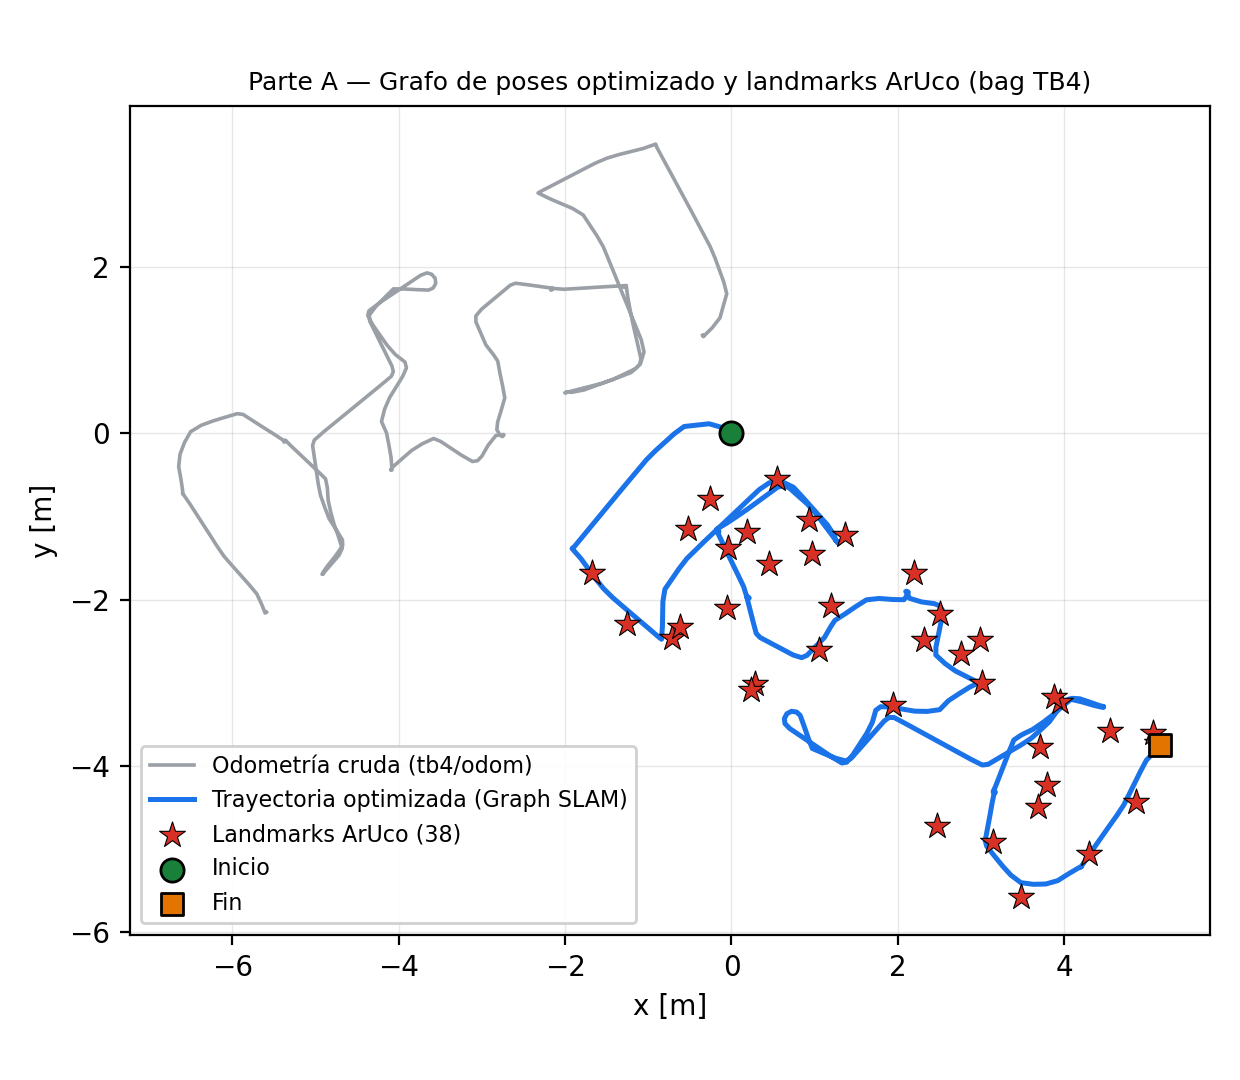
\includegraphics[width=0.90\columnwidth]{parte_a_trajectory.png}
\caption{Parte~A: grafo de poses optimizado (azul) frente a la odometría cruda del TB4 (gris) y los 38 landmarks ArUco estimados (estrellas rojas). La deriva odométrica de varios metros se corrige por las re-observaciones de marcadores.}
\label{fig:parte_a_traj}
\end{figure}

\begin{figure}[t]
\centering
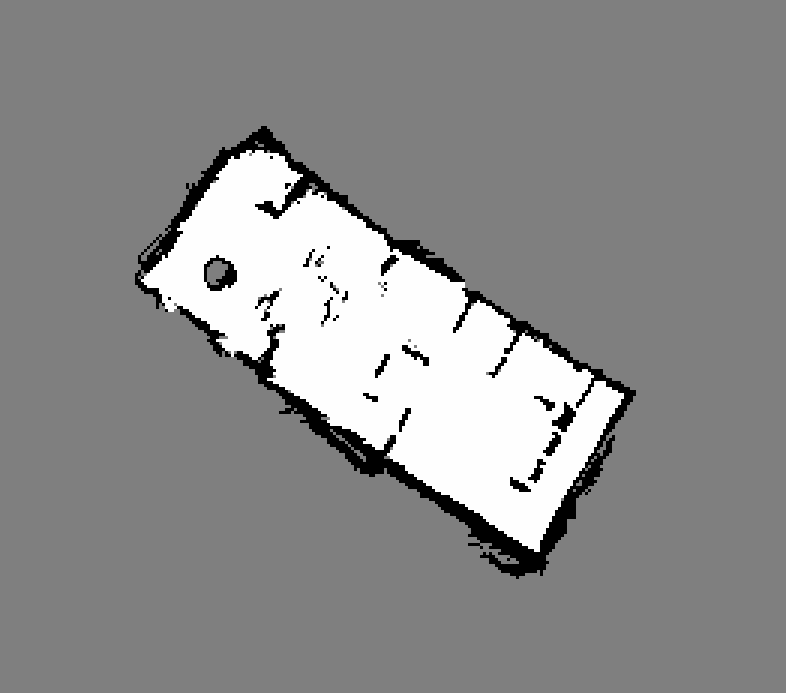
\includegraphics[width=0.72\columnwidth]{mapa_tb4_real.png}
\caption{Grilla de ocupación del laberinto real (bag TB4) generada en la segunda pasada: $262\times231$ celdas a $0.05$~m. Negro: ocupado; blanco: libre; gris: desconocido.}
\label{fig:parte_a_map}
\end{figure}

Para verificar la estabilidad del mapeo evaluamos el efecto del \emph{bracketing} de TF y del gate angular sobre un bag largo (1392.8~s, 10\,797 barridos). La Tabla~\ref{tab:mapa_comparacion} resume la comparación entre desactivar y activar el gate angular: ambas variantes integran prácticamente todos los barridos usando la TF real (un único \emph{fallback} por corrida), producen la misma cantidad de celdas ocupadas y difieren en una sola celda, confirmando que el \emph{bracketing} elimina el \emph{clamp} al último odom sin necesitar cambios de log-odds. Se conserva el gate desactivado por defecto.

\begin{table}[h]
\centering
\caption{Estabilidad del mapeo (bag largo, 10\,797 barridos)}
\label{tab:mapa_comparacion}
\begin{tabular}{lcc}
\toprule
\textbf{Métrica} & \textbf{Sin gate} & \textbf{Gate 0.35} \\
\midrule
Barridos integrados & 10\,770 & 10\,783 \\
Descartados por giro & 0 & 1 \\
TF real / fallback & 10\,769/1 & 10\,782/1 \\
Máximo gap odométrico & 946.9 ms & 590.1 ms \\
Celdas ocupadas & 2\,058 & 2\,058 \\
Espesor de pared (mediana/p95) & 0.10/0.28 m & 0.10/0.28 m \\
Celdas distintas entre mapas & \multicolumn{2}{c}{1} \\
\bottomrule
\end{tabular}
\end{table}

La Tabla~\ref{tab:params_a} reúne los parámetros de diseño más relevantes de la Parte~A.

\begin{table}[h]
\centering
\caption{Parámetros clave de la Parte A}
\label{tab:params_a}
\begin{tabular}{lll}
\toprule
\textbf{Módulo} & \textbf{Parámetro} & \textbf{Valor} \\
\midrule
Keyframe & distancia / ángulo & 0.15 m / 0.60 rad \\
Odometría & $\boldsymbol{\sigma}$ (x,y,$\theta$) & 0.3, 0.3, 0.1 \\
Avistaje & $\sigma_\phi(r),\sigma_r(r)$ & $0.10{+}0.05r$ / $0.024{+}0.032r^2$ \\
Optimizador & método / kernel & LM / Cauchy $k{=}1$ \\
Cierre lazo & paralaje / salto / $\chi^2$ & 0.20 m / 0.75 m / 5.99 \\
ArUco & área mín / reproj. máx & 250 px / 4.0 px \\
Grilla & resolución & 0.05 m/celda \\
Grilla & $L_{\text{occ}}/L_{\text{free}}$ & $+0.85$ / $-0.40$ \\
\bottomrule
\end{tabular}
\end{table}


%=================================================================
% PARTE B
%=================================================================
\section{Parte B: Navegación Autónoma (Sistema 3)}
\label{sec:parte_b}

La Parte~B implementa la navegación autónoma sobre el mapa consolidado, siguiendo el \emph{Sistema~3} de la consigna (grilla de ocupación + landmarks de cámara). Como Gazebo no provee marcadores visuales nativos, diseñamos un \textbf{sensor virtual de landmarks} que emula el detector ArUco. Todo el código nuevo reside en el paquete \texttt{tp\_b\_navigation}, sin modificar la Parte~A.

\subsection{Arquitectura de nodos y cadena de TF}
El sistema se descompone en siete nodos con responsabilidades claras (Fig.~\ref{fig:nodos_b}). La decisión de diseño central es que \textbf{un único nodo, la máquina de estados, es el dueño exclusivo de \texttt{/cmd\_vel}}: fusiona la FSM con el controlador de seguimiento, el ángulo final y la evasión, porque coordinar el control entre procesos es mucho más frágil que tener un único productor de velocidad. El planificador y el monitor de obstáculos quedan como nodos puros, separados para claridad.

\begin{figure}[t]
\centering
\begin{tikzpicture}[node distance=3mm and 4mm]
  \node[node2] (map) {map\_loader};
  \node[node2, right=8mm of map] (lmp) {landmark\_pub.};
  \node[node2, below=of map] (sensor) {landmark\_sensor};
  \node[node2, right=of sensor] (mcl) {mcl\_localization};
  \node[node2, below=of mcl] (plan) {global\_planner};
  \node[node2, left=of plan] (mon) {obstacle\_monitor};
  \node[state, below=6mm of plan] (fsm) {state\_machine\\\textbf{/cmd\_vel}};
  \draw[tr] (map) -- node[left,topic]{/map} (sensor);
  \draw[tr] (lmp) -- node[right,topic]{/landmarks} (mcl);
  \draw[tr] (sensor) -- node[above,topic]{obs} (mcl);
  \draw[tr] (mcl) -- node[left,topic]{TF map$\to$odom} (plan);
  \draw[tr] (plan) -- node[right,topic]{/plan} (fsm);
  \draw[tr] (mon) -- node[left,topic]{/obstacle} (fsm);
  \draw[tr] (fsm) to[bend left=30] node[right,topic]{/plan\_request} (plan);
\end{tikzpicture}
\caption{Mapa de nodos de la Parte~B. El MCL cierra la cadena de TF publicando \texttt{map$\to$odom}; la máquina de estados es el único productor de \texttt{/cmd\_vel}.}
\label{fig:nodos_b}
\end{figure}

La cadena de transformadas es \texttt{map}\,$\to$\,\allowbreak\texttt{odom}\,$\to$\,\allowbreak\texttt{base\_footprint}\,$\to$\,\allowbreak\texttt{base\_scan}. Gazebo publica \texttt{odom}\,$\to$\,\texttt{base\_footprint}; el \textbf{MCL cierra la cadena} publicando la corrección \texttt{map}\,$\to$\,\texttt{odom} a 30~Hz. Todos los consumidores leen la pose del robot con \texttt{lookup\_transform(map, base\_footprint)}.

\subsection{Localización: filtro de partículas (MCL)}
El nodo \texttt{mcl\_localization} implementa \emph{Monte Carlo Localization} \cite{amcl} con mapa y landmarks conocidos y fijos (no hace SLAM). Usa $N=350$ partículas, inicializadas por la herramienta ``2D Pose Estimate'' de RViz (\texttt{/initialpose}).

\textbf{Predicción:} por cada mensaje de \texttt{/calc\_odom} se aplica el modelo de movimiento por odometría (deltas $\delta_{\text{rot1}},\delta_{\text{trans}},\delta_{\text{rot2}}$ con ruido $\alpha_{1..4}$). La odometría de referencia de Gazebo se mantiene separada sólo para construir la TF \texttt{map$\to$odom}.

\textbf{Corrección híbrida:} las partículas se pesan combinando dos modelos de medición:
\begin{itemize}
\item \emph{Láser--mapa}: se construye un \emph{likelihood field} desde las celdas ocupadas del mapa y se pondera según cuán cerca caen de las paredes los \emph{endpoints} muestreados del LIDAR (hasta 60 haces, $\sigma_{\text{hit}}=0.18$~m). Partículas fuera del mapa, en desconocido o dentro de ocupado reciben una penalización fuerte.
\item \emph{Landmarks}: acepta tanto el contrato por índice (\texttt{/observed\_landmarks}) como el identificado por ID ArUco (\texttt{/observed\_landmark\_ids}); en el bag/real la asociación es directa contra los IDs del \texttt{trajectory.json} de la Parte~A.
\end{itemize}
Las correcciones se disparan sólo tras movimiento suficiente ($\texttt{update\_min\_d}/\texttt{update\_min\_a}$) para evitar la degeneración estática de la nube.

\textbf{Remuestreo y diversidad:} se usa remuestreo de baja varianza cuando $n_{\text{eff}}<N/2$, seguido de \emph{roughening} (jitter $0.03$~m en posición, $0.02$~rad en ángulo) para evitar el empobrecimiento de partículas. Finalmente, la TF \texttt{map$\to$odom} se publica con la estampa adelantada $0.1$~s (\texttt{transform\_tolerance}, truco de AMCL) para que siga siendo válida ante lecturas con estampa más nueva, evitando el parpadeo por ``extrapolation into the future''.

\subsection{Sensor virtual de landmarks con oclusión}
El nodo \texttt{landmark\_sensor} emula el detector ArUco ausente en Gazebo. Por cada landmark conocido: (1)~lo proyecta al marco del robot y calcula \emph{range}+\emph{bearing}; (2)~descarta los que caen fuera del FOV de $1.05$~rad o del rango; (3)~calcula la \textbf{oclusión por línea de visión} comparando el \emph{range} esperado contra el rayo central del LIDAR (si un obstáculo aparece $>0.08$~m antes, el landmark está ocluido y no se publica); (4)~agrega ruido gaussiano ($\sigma_r=\sigma_\phi=0.05$).

Dos decisiones fueron críticas para la convergencia:
\begin{itemize}
\item \textbf{Desacople de la estimación (\texttt{truth\_frame}):} una cámara real ve los landmarks según la pose \emph{verdadera} del robot, no según la estimación del filtro. Proyectar con la TF del MCL realimentaría el filtro consigo mismo y lo haría diverger. Por eso el sensor proyecta con \texttt{odom$\to$base} (en Gazebo la odometría es cuasi \emph{ground-truth}).
\item \textbf{Estampa de la TF, no del scan:} la salida se estampa con el tiempo de la TF usada, no con el del \texttt{/scan} (que Gazebo adelanta 20--60~ms), garantizando una cadena \texttt{map$\to$odom$\to$base} válida en ese instante.
\end{itemize}

\textbf{Densidad de landmarks:} la consigna pide una densidad ``coherente con el ArUco real''. Escalamos de 14 a 36 y finalmente a \textbf{60 landmarks}, distribuidos por \emph{farthest-point sampling} sobre superficies de pared (un landmark en espacio libre nunca devolvería eco del LIDAR y jamás sería ``visible''). Con pocos landmarks el posterior se volvía multimodal por las simetrías de la casa (§\ref{sub:tuning}).

\subsection{Planificación global: A$^\star$}
El \texttt{global\_planner} ejecuta A$^\star$ 8-conexo \cite{astar} sobre la grilla, con: \textbf{inflado} de obstáculos por el radio del robot ($0.18$~m, distancia de Chebyshev por BFS multi-fuente); \textbf{penalización de cercanía} (\emph{clearance}) que encarece pasar pegado a las paredes, de modo que el robot prefiere el centro de los pasillos; tratamiento de las celdas desconocidas como obstáculo (\texttt{allow\_unknown=False}, por seguridad); y un \textbf{atajo por línea de visión} (Bresenham) que simplifica la ruta a pocos \emph{waypoints}, forzando el último exactamente al \texttt{goal\_pose}. Es un nodo puro: planifica al recibir \texttt{/plan\_request} y publica \texttt{/plan}.

\subsection{Seguimiento, ángulo final y obstáculos}
El seguimiento usa \textbf{pure-pursuit} \cite{purepursuit} con un punto ``zanahoria'' a \texttt{lookahead}$=0.30$~m: el rumbo se corrige con ganancia $k_w=1.6$ y la velocidad lineal se reduce con el error angular, $v=v_{\max}\max(0,1-|e|/\text{slow\_angle})$, de modo que el robot gira primero y avanza suave ($v_{\max}=0.18$~m/s, $w_{\max}=1.2$~rad/s). Alcanzada la posición (\texttt{goal\_xy\_tol}$=0.12$~m), un estado dedicado gira en el lugar hasta el \textbf{ángulo final} (\texttt{goal\_yaw\_tol}$=0.08$~rad).

Para \textbf{obstáculos no mapeados}, el \texttt{obstacle\_monitor} distingue paredes conocidas de obstáculos nuevos: por cada eco del LIDAR en un cono frontal ($0.6$~rad) y cercano ($<0.45$~m), proyecta el punto a \texttt{map} y consulta la celda; si el mapa la marca libre pero el LIDAR ve algo, es un obstáculo nuevo. Con $\geq 3$ puntos nuevos publica \texttt{/obstacle\_detected}, y conserva los puntos en \texttt{/dynamic\_obstacles} (con inflación compacta de $0.08$~m) para que el siguiente A$^\star$ los rodee sin clausurar todo el pasillo.

\subsection{Máquina de estados}
La Fig.~\ref{fig:fsm_b} muestra el diagrama de bloques de la máquina de estados de la Parte~B, que gobierna el ciclo completo con ocho estados. El flujo nominal es \texttt{IDLE}\,$\to$\,\allowbreak\texttt{LOCALIZING}\,$\to$\,\allowbreak\texttt{WAITING\_GOAL}\,$\to$\,\allowbreak\texttt{PLANNING}\,$\to$\,\allowbreak\texttt{FOLLOWING}\,$\to$\,\allowbreak\texttt{ALIGNING\_ANGLE}\,$\to$\,\allowbreak\texttt{GOAL\_REACHED}. Las ramas cubren la evasión (\texttt{AVOIDING}), el re-planeo ante un nuevo objetivo en cualquier estado activo (requisito~1.8) y el fallo/\emph{timeout} de planificación. Un \texttt{/initialpose} reinicia siempre a \texttt{LOCALIZING}.

\begin{figure}[t]
\centering
\begin{tikzpicture}[node distance=6mm and 9mm]
  \node[state] (idle) {IDLE};
  \node[state, below=of idle] (loc) {LOCALIZING};
  \node[state, below=of loc] (wait) {WAITING\_GOAL};
  \node[state, right=14mm of wait] (plan) {PLANNING};
  \node[state, above=of plan] (follow) {FOLLOWING};
  \node[state, right=10mm of follow] (avoid) {AVOIDING};
  \node[state, above=of follow] (align) {ALIGNING\_ANGLE};
  \node[term, above=of align] (reached) {GOAL\_REACHED};
  \draw[tr] (idle) -- node[left]{initialpose} (loc);
  \draw[tr] (loc) -- node[left]{TF estable 1.5s} (wait);
  \draw[tr] (wait) -- node[below]{goal\_pose} (plan);
  \draw[tr] (plan) -- node[right]{plan OK} (follow);
  \draw[tr] (plan.south) to[bend right=20] node[below,align=center]{plan falla\\/timeout} (wait.east);
  \draw[tr] (follow) -- node[above]{obstáculo} (avoid);
  \draw[tr] (avoid) to[bend left=25] node[right]{despejado} (plan);
  \draw[tr] (follow) -- node[right]{llegó (xy)} (align);
  \draw[tr] (align) -- node[right]{yaw OK} (reached);
  \draw[tr] (reached.west) to[bend right=55] node[left]{listo} (wait.north);
  \draw[tr] (follow.west) to[bend right=12] node[left,pos=0.4]{goal nuevo} (plan.north west);
\end{tikzpicture}
\caption{Diagrama de bloques de la máquina de estados de la Parte~B. Cada arco indica el evento o condición que dispara la transición. Un \texttt{/initialpose} (no dibujado desde todos los orígenes) reinicia a \texttt{LOCALIZING}, y un \texttt{goal\_pose} nuevo re-planifica desde cualquier estado activo.}
\label{fig:fsm_b}
\end{figure}

\subsection{Resultados y bitácora de \emph{tuning}}
\label{sub:tuning}

\textbf{Ciclo completo en \texttt{custom\_casa}.} Con localización perfecta (TF identidad, para aislar la navegación), el robot fue a un \emph{goal} a $180^\circ$ y llegó con error $\sim$10~cm/$3^\circ$, rodeando correctamente la sala central. Con el \textbf{MCL real}, cruzó toda la casa ($\sim$5~m) y llegó con error $\sim$6~cm, con el MCL estimando a $\sim$1.5~cm de la pose real en el \emph{goal} (Fig.~\ref{fig:nav_b}).

\begin{figure}[t]
\centering
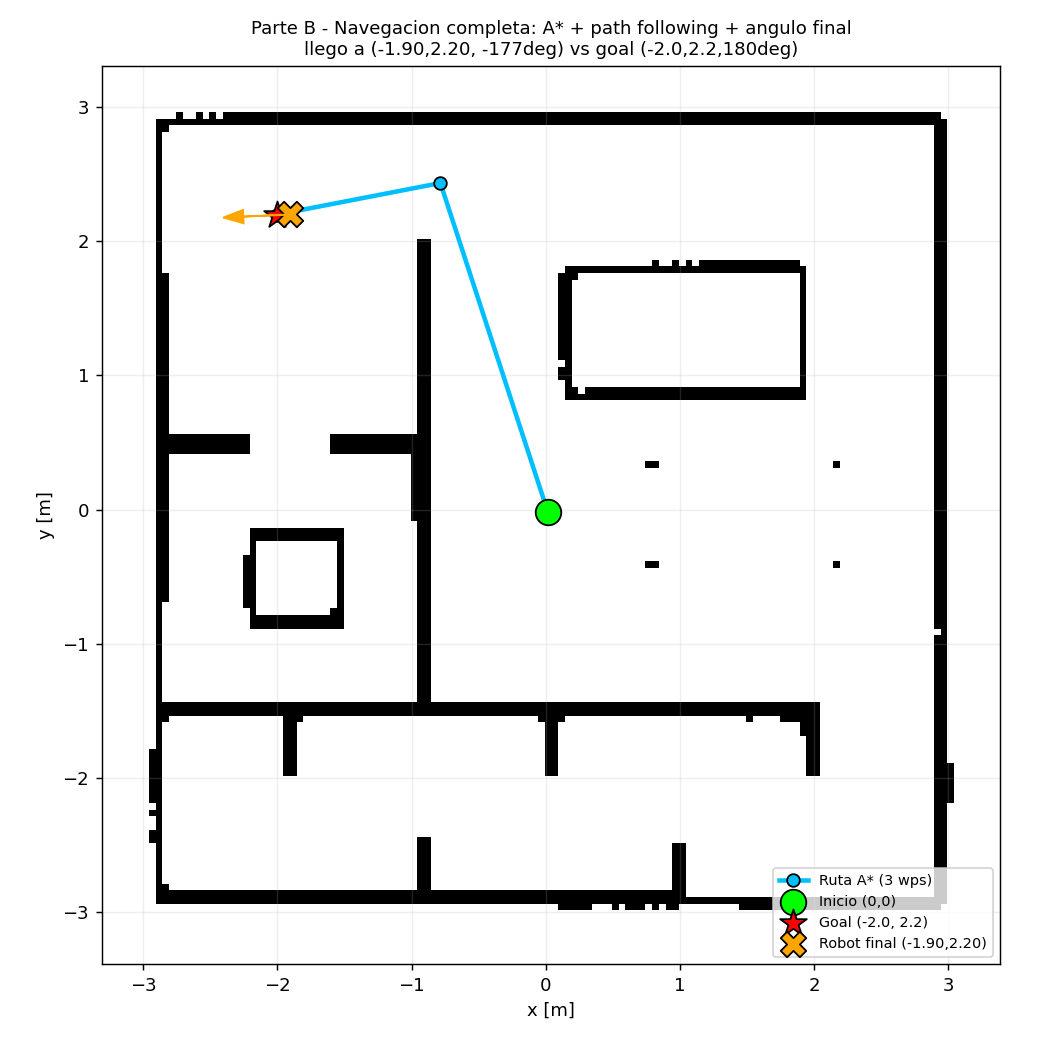
\includegraphics[width=0.85\columnwidth]{02_navegacion_localizacion_perfecta.png}
\caption{Navegación en \texttt{custom\_casa}: ruta A$^\star$ (verde) que rodea la sala central, trayectoria seguida y \emph{goal} alcanzado con ángulo final.}
\label{fig:nav_b}
\end{figure}

\textbf{Convergencia del MCL.} El MCL inicialmente divergía. Tres correcciones, cada una verificada con datos, lo estabilizaron (Tabla~\ref{tab:tuning_mcl}): (1)~desacoplar el sensor de la estimación; (2)~elevar la densidad de 14 a 36--60 landmarks para eliminar la multimodalidad; (3)~\emph{roughening} + 350 partículas para recuperarse de discrepancias transitorias en lugar de diverger.

\begin{table}[h]
\centering
\caption{Tuning del MCL: antes vs.\ después}
\label{tab:tuning_mcl}
\begin{tabular}{lccc}
\toprule
\textbf{Config.} & \textbf{Err. medio} & \textbf{Err. máx} & \textbf{Comportamiento} \\
\midrule
Antes (14 lm, acoplado) & 0.65 m & 2.9 m & diverge \\
Después (36--60 lm, rough.) & \textbf{0.02--0.18 m} & recupera & trackea pegado \\
\bottomrule
\end{tabular}
\end{table}

\textbf{Obstáculos no mapeados en \texttt{custom\_casa\_obs}.} Con un \emph{goal} cuya ruta cruza una valija no mapeada, el monitor la detectó correctamente, la FSM entró en \texttt{AVOIDING} (8 maniobras), el robot \textbf{esquivó sin chocar} y el MCL se mantuvo preciso durante las rotaciones (error medio $0.16$~m, máx $0.90$~m sobre 799 muestras). Con \emph{goals} que no cruzan obstáculos no hubo falsos positivos (Fig.~\ref{fig:evasion_b}).

\begin{figure}[t]
\centering
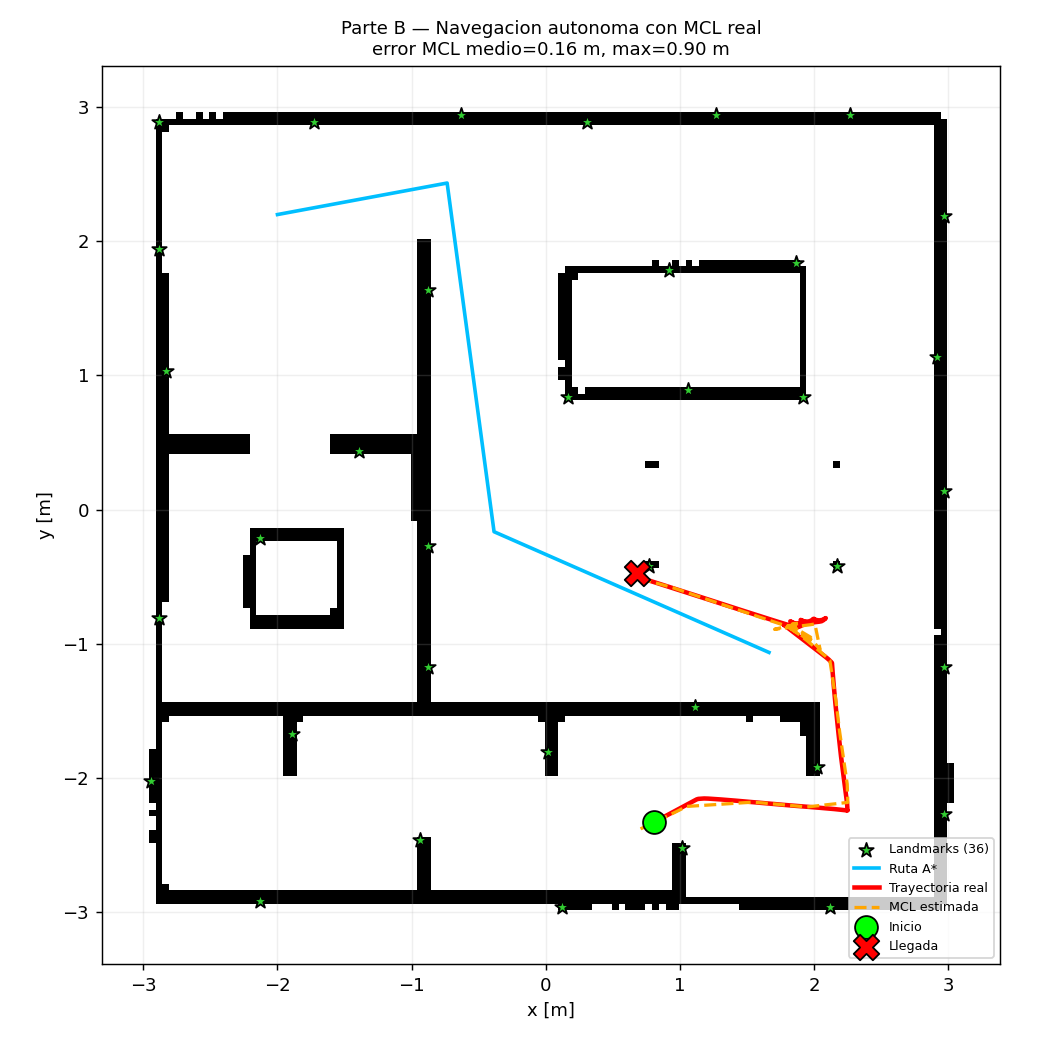
\includegraphics[width=0.85\columnwidth]{04_evasion_obstaculos.png}
\caption{Evasión en \texttt{custom\_casa\_obs}: el robot detecta la valija no mapeada, la esquiva (trayectoria roja) sin colisión y el MCL (naranja) se mantiene pegado a la pose real.}
\label{fig:evasion_b}
\end{figure}

\textbf{Limitación conocida.} Cuando un obstáculo se sienta \emph{justo} sobre la única ruta buena (p.\,ej.\ un \emph{cluster} tapando la entrada al cuarto del \emph{goal}), la navegación se vuelve lenta y sinuosa: el planificador razona sobre el mapa estático y re-planifica la misma ruta bloqueada, avanzando sólo por los empujones reactivos de \texttt{AVOIDING}. No choca ni se rompe, pero es ineficiente. La mejora natural es un \emph{costmap local} que sume los obstáculos detectados al mapa estático para que A$^\star$ los rodee. La Tabla~\ref{tab:consigna_b} resume el cumplimiento de la consigna.

\begin{table}[h]
\centering
\caption{Cumplimiento de la consigna de Parte B}
\label{tab:consigna_b}
\begin{tabular}{ll}
\toprule
\textbf{Requisito} & \textbf{Estado} \\
\midrule
1.1 Sistema 3 (landmarks de cámara) & \checkmark\ 60 lm + oclusión \\
1.2 Localización inicial (\texttt{initialpose}) & \checkmark \\
1.4 Localización continua (filtro prob.) & \checkmark\ MCL 0.02--0.18 m \\
1.5 Planificación (A$^\star$/inflado/seguro) & \checkmark \\
1.6 Seguimiento suave & \checkmark\ pure-pursuit \\
1.7 Ángulo final & \checkmark \\
1.8 Re-planeo (goal nuevo) & \checkmark \\
1.9 Obstáculos no mapeados & $\triangle$ esquiva; ineficiente si tapa ruta \\
1.11 Máquina de estados & \checkmark\ FSM completa \\
\bottomrule
\end{tabular}
\end{table}

\textbf{Re-mapeo del entorno simulado.} Como pide el Sistema~3, no reutilizamos el mapa del RosBag (mundo distinto), sino que repetimos el mapeo en Gazebo con el nodo \texttt{sim\_mapper}, que porta el núcleo de la grilla de ocupación de la Parte~A (mismas constantes de log-odds y export) pero toma la pose de cada barrido de la TF en vivo. El mapa generado por teleoperación ($220\times220$ a $0.05$~m) cubre el 100\% de las paredes con alineación casi perfecta respecto del mapa de referencia.


%=================================================================
% PARTE C
%=================================================================
\section{Parte C: Despliegue Real, Exploración Informativa y Percepción}
\label{sec:parte_c}

La Parte~C lleva el sistema al robot físico y le añade una \textbf{misión de exploración activa}: recorrer autónomamente el laberinto buscando conos rojos, discriminándolos de distractores de otros colores y aproximándose sin intentar atravesar paredes. La capa de misión (paquete \texttt{tp\_c\_mission}) se monta \emph{encima} de la navegación estable de la Parte~B sin reemplazarla: el \texttt{mission\_manager} nunca produce \texttt{/cmd\_vel}, sino que publica objetivos en \texttt{/mission\_goal} y deja que la máquina de estados de la Parte~B ejecute el movimiento (Fig.~\ref{fig:c_arch}).

\begin{figure}[t]
\centering
\begin{tikzpicture}[node distance=5mm and 7mm]
  \node[node2] (cone) {red\_cone\_detector};
  \node[node2, right=of cone] (mm) {mission\_manager\\(exploración)};
  \node[state, below=of mm] (fsm) {state\_machine\\(Parte B)};
  \node[node2, left=of fsm] (mcl) {mcl\_localization};
  \draw[tr] (cone) -- node[above,topic]{/red\_cone\_pose} (mm);
  \draw[tr] (mm) -- node[right,topic]{/mission\_goal} (fsm);
  \draw[tr] (fsm) to[bend left=35] node[right,topic]{/navigation\_result} (mm);
  \draw[tr] (mcl) -- node[below,topic]{/mcl\_pose} (fsm);
  \draw[tr] (mcl) to[bend right=20] node[left,topic]{pose+cov} (mm);
\end{tikzpicture}
\caption{Arquitectura de la Parte~C. La misión decide \emph{a dónde} ir y la FSM de la Parte~B decide \emph{cómo} moverse; la realimentación viaja por \texttt{/navigation\_result}.}
\label{fig:c_arch}
\end{figure}

\subsection{Exploración informativa}
El \texttt{mission\_manager} mantiene una creencia de cobertura (\texttt{CoverageBelief}) de qué celdas libres ya fueron observadas por la cámara. En cada ciclo genera poses candidatas alcanzables (barrido de la grilla con paso $0.50$~m, 8 orientaciones por celda) y, para cada una, estima por \emph{ray-casting} qué celdas vería la cámara (FOV $1.05$~rad, alcance $3.0$~m; la visibilidad se precalcula una vez por mapa). Selecciona la acción que maximiza una \textbf{función de utilidad}:
\begin{equation}
U = 0.55\,g_{\text{cob}} + 0.20\,g_{\text{loc}}\,s_{\text{cov}} - 0.20\,c_{\text{cam}} - 0.05\,(\rho+\text{rep}),
\end{equation}
donde $g_{\text{cob}}$ es la ganancia de cobertura (celdas nuevas normalizadas), $g_{\text{loc}}$ la fracción de landmarks de la Parte~A que quedarían visibles (mejora la localización), $s_{\text{cov}}$ un factor que pesa más la localización cuando la incertidumbre del MCL es alta, $c_{\text{cam}}$ el costo del camino A$^\star$ normalizado, $\rho$ el riesgo por cercanía a obstáculos y \emph{rep} una penalización a celdas ya visitadas. El costo del camino se refina con A$^\star$ sólo para los mejores candidatos por un \emph{ranking} barato previo. Si no hay acciones informativas o la cobertura supera el 95\%, la misión termina en \texttt{NOT\_FOUND}; existe además un \emph{fallback} de frontera que prioriza celdas libres no observadas adyacentes a lo ya visto.

\subsection{Detección de conos rojos}
El nodo \texttt{red\_cone\_detector} resuelve los dos desafíos que plantea la consigna: discriminar el rojo de distractores y no ``ver a través'' de las paredes.

\textbf{Segmentación en HSV (dos bandas):} el rojo envuelve el origen del matiz, por lo que la máscara combina dos bandas ($H\leq 10$ \emph{o} $H\geq 170$ en escala OpenCV) con saturación $\geq 100$ y valor $\geq 70$. La máscara se limpia con apertura + cierre morfológico.

\textbf{Validación geométrica:} sobre las componentes conexas se exige área $\geq 150$~px, altura $\geq 10$~px, un factor de llenado $\geq 0.20$ y \textbf{forma de cono} (base más ancha que la punta). Con \emph{depth} real se añade validación 3D que descarta distractores planos (como una superficie roja): se estima la altura real del objeto y se rechaza si difiere $>0.13$~m de los $\sim$0.30~m del cono, o si su base no está apoyada en el piso ($|z|>0.20$~m).

\textbf{Confirmación temporal:} un rastreador exige $\geq 3$ detecciones en una ventana de 5 \emph{frames} con centros consistentes ($<25$~px de salto) antes de confirmar, filtrando destellos espurios.

\textbf{Estimación de distancia (con degradación elegante):} se prefiere la mediana del \emph{depth} alineado sobre los píxeles del cono ($\sigma=0.05$~m); si no hay \emph{depth} válido, se usa el \emph{fallback} monocular $d = f_y\,h_{\text{cono}}/h_{\text{px}}$ ($\sigma=0.20$~m); en el robot real se usan además haces del LIDAR en la dirección del cono. La detección confirmada se publica como \texttt{/red\_cone\_pose} en el marco \texttt{map}, con covarianza acorde a la fuente.

Crucialmente, la detección \textbf{nunca se convierte en un comando de velocidad}: reporta la coordenada al planificador, que genera una trayectoria válida que rodea los muros reales (si el cono se ve por una abertura, el objetivo se valida sobre la grilla). Sólo se acepta una pose de aproximación libre, visible y alcanzable por A$^\star$ (anillo de \emph{standoff} $0.55$~m alrededor del cono).

\subsection{Adaptador ArUco$\rightarrow$MCL para el robot real}
En el robot físico no hay sensor virtual: las detecciones ArUco reales las procesa \texttt{aruco\_mcl\_adapter}, que transforma cada marcador a \emph{range}/\emph{bearing} con su ID y compensa la latencia de la imagen. Un hallazgo de laboratorio fue que la imagen RGB podía llegar al \emph{callback} 2.6--2.9~s después de su estampa, mientras el LIDAR llegaba fresco; el adaptador re-expresa la observación de \texttt{base}$(t_{\text{obs}})$ a \texttt{base}$(t_{\text{ahora}})$ usando el movimiento relativo en \texttt{odom} antes de publicarla. El MCL asocia entonces la observación por ID directamente contra las posiciones optimizadas del \texttt{trajectory.json} de la Parte~A, sin \emph{data association} geométrica.

\subsection{Máquina de estados de la misión}
La Fig.~\ref{fig:fsm_c} muestra el diagrama de bloques de la máquina de estados de la misión (Parte~C). Desde \texttt{IDLE}, el servicio \texttt{/mission/start} --- que sólo procede si hay mapa, pose MCL fresca y visión lista --- pasa a \texttt{EXPLORING}. Una detección confirmada alcanzable dispara \texttt{APPROACHING}; al alcanzar el cono (\texttt{/navigation\_result = REACHED}) la misión termina en \texttt{FOUND}. Un plan fallido de aproximación vuelve a \texttt{EXPLORING}. Los estados terminales \texttt{NOT\_FOUND} (\emph{timeout} o cobertura agotada) y \texttt{FAILED} (gate de seguridad, ver abajo) cierran la misión y detienen la navegación.

\begin{figure}[t]
\centering
\begin{tikzpicture}[node distance=7mm and 12mm]
  \node[state] (idle) {IDLE};
  \node[state, right=of idle] (exp) {EXPLORING};
  \node[state, right=of exp] (app) {APPROACHING};
  \node[term, below=8mm of app] (found) {FOUND};
  \node[term, below=8mm of exp] (nf) {NOT\_FOUND};
  \node[term, below=8mm of idle] (fail) {FAILED};
  \draw[tr] (idle) -- node[above,align=center]{start\\(gates OK)} (exp);
  \draw[tr] (exp) -- node[above]{cono visible} (app);
  \draw[tr] (app) to[bend left=25] node[below]{plan falla} (exp);
  \draw[tr] (app) -- node[right]{REACHED} (found);
  \draw[tr] (exp) -- node[right,align=center]{timeout /\\cobertura} (nf);
  \draw[tr] (exp) to[bend right=12] node[left,pos=0.3]{gate/visión} (fail);
  \draw[tr] (idle) -- node[left]{start bloq.} (fail);
\end{tikzpicture}
\caption{Diagrama de bloques de la máquina de estados de la misión de la Parte~C. Los estados verdes son terminales. La cancelación (\texttt{/mission/cancel}) retorna a \texttt{IDLE} desde cualquier estado activo (no dibujada).}
\label{fig:fsm_c}
\end{figure}

\subsection{Gates de seguridad}
En el perfil real, la misión aborta a \texttt{FAILED} y publica velocidad cero si la pose del MCL queda vieja ($>1.0$~s), su covarianza supera los umbrales ($0.25$~m$^2$ en posición, $0.5$ en \emph{yaw}) o la visión/TF de cámara deja de estar fresca ($>3.0$~s). Estos \emph{gates} también bloquean el arranque de la misión. Es una salvaguarda deliberada para el hardware: ante duda sobre dónde está el robot, se detiene.

\subsection{Validación y estado (a completar)}
Siguiendo la metodología exigida por la consigna, validamos exhaustivamente contra RosBags antes del laboratorio. Los tests unitarios de percepción, exploración y contratos pasan sin ROS; el \emph{smoke} conjunto sobre el bag del laberinto (transporte, predicción del MCL y salud del monitor) aprueba 3 pruebas y la suite ROS 215 pruebas, sin publicar jamás sobre el \texttt{/cmd\_vel} físico. La Fig.~\ref{fig:c_explore} ilustra la cobertura explorada y los \emph{frontiers} candidatos en simulación.

\begin{figure}[t]
\centering
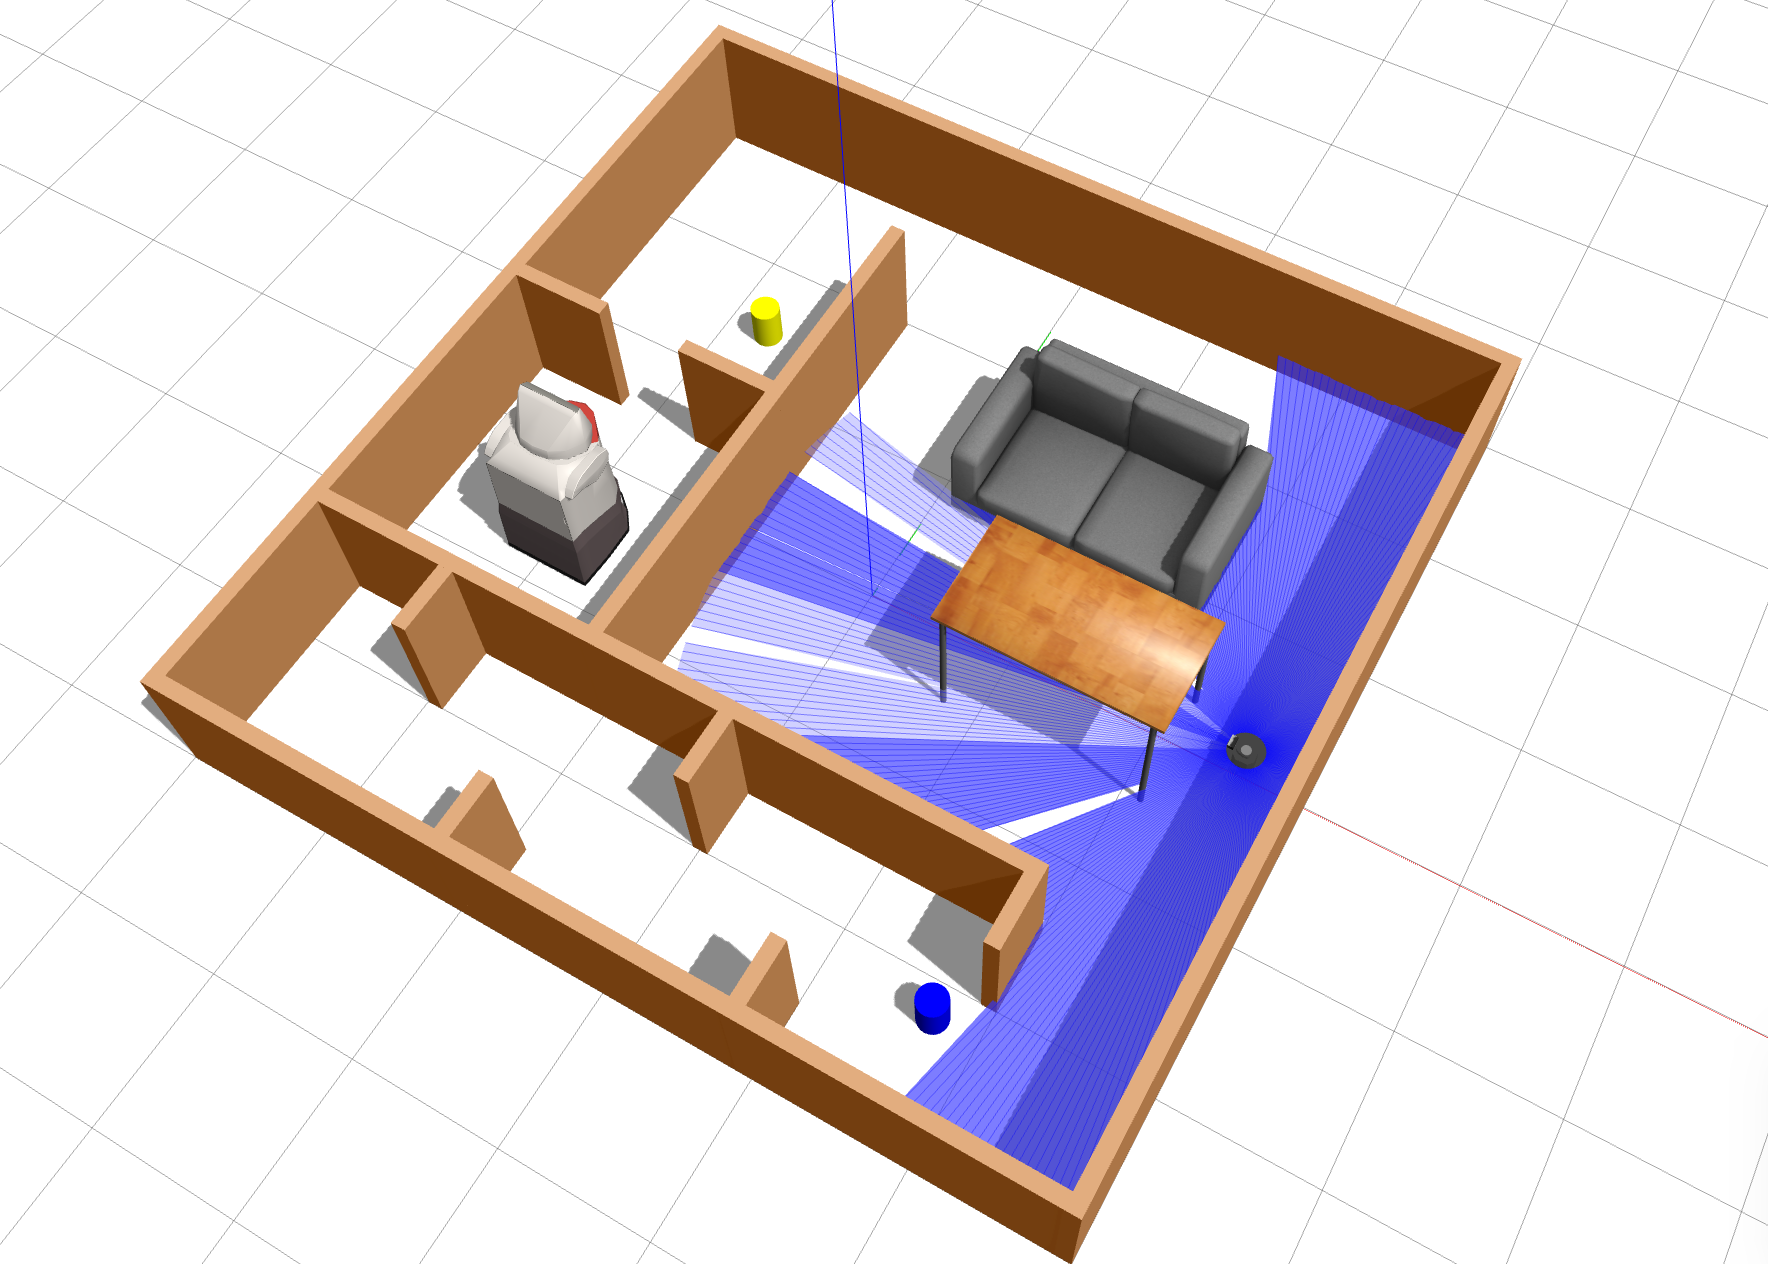
\includegraphics[width=0.85\columnwidth]{exploring.png}
\caption{Exploración informativa en simulación: cobertura observada por la cámara (celdas) y candidatos \emph{frontier} evaluados por la función de utilidad.}
\label{fig:c_explore}
\end{figure}

\textbf{Pendiente de hardware.} Al momento de esta redacción \emph{no se realizó todavía la prueba sobre el robot físico}. Quedan pendientes los \emph{gates} físicos, que se ejecutarán en la ventana de laboratorio con el robot detenido y la parada de emergencia accesible: (B1)~localización con movimiento deshabilitado; (B2)~un \emph{goal} corto a velocidad reducida y luego múltiples \emph{goals}; (B3)~detección de obstáculo con el robot detenido, re-planeo sin movimiento y evasión reducida con recuperación del MCL. El análisis cuantitativo de la brecha \emph{sim-to-real} y los resultados de la misión de conos sobre hardware se incorporarán tras esa sesión (§\ref{sec:conclusion}).


%=================================================================
% DISCUSION Y CONCLUSION
%=================================================================
\section{Discusión y Brecha Sim-to-Real}
\label{sec:conclusion}

El hilo conductor de las tres partes fue la \textbf{gestión rigurosa de la incertidumbre y del tiempo}. Varias de las decisiones de diseño más importantes no surgieron de la teoría sino de patologías observadas sobre datos reales o simulados: el desacople del sensor virtual de la estimación del filtro (sin el cual el MCL se realimentaba y divergía), el \emph{bracketing} temporal que nunca extrapola (que eliminó el emborronamiento de las paredes en el mapa), la compensación de la latencia de la imagen ArUco (2.6--2.9~s en el laboratorio) y el kernel robusto de Cauchy sobre los avistajes (que evita que un falso cierre de lazo arruine el grafo). Documentarlas es, a nuestro juicio, tan valioso como el resultado final.

\textbf{Sobre la brecha sim-to-real.} La arquitectura fue diseñada explícitamente para minimizar esta brecha: la Parte~B corre sobre landmarks \emph{virtuales} calibrados en densidad y con oclusión geométrica para plantear ``un desafío matemático equivalente'' al del ArUco real, y el mismo nodo MCL acepta tanto los IDs virtuales de simulación como los IDs ArUco reales del \texttt{trajectory.json}. Los factores que anticipamos como principales fuentes de discrepancia en el robot físico son: (i)~el ruido y la deriva reales de la odometría del Create~3 frente a la odometría cuasi-perfecta de Gazebo; (ii)~la latencia y el \emph{motion blur} de la cámara OAK-D; (iii)~los cambios de iluminación del laboratorio sobre la segmentación HSV de los conos; y (iv)~el deslizamiento mecánico. Los \emph{gates} de seguridad y la compensación de latencia son las defensas preparadas de antemano contra (i)--(ii).

\textbf{Limitaciones.} (1)~El planificador razona sobre el mapa estático, por lo que un obstáculo denso sobre la única ruta produce navegación ineficiente (falta un \emph{costmap local}). (2)~El cierre de lazo de la Parte~A depende de la re-observación de marcadores; en tramos largos sin ArUco visible la deriva sólo se corrige al reencontrar un marcador. (3)~La validación del sistema completo en hardware está pendiente de la ventana de laboratorio.

\section{Conclusión y Trabajo Futuro}

Presentamos la memoria técnica de un sistema robótico autónomo completo que integra SLAM visual con Graph SLAM y marcadores ArUco (Parte~A), navegación autónoma con localización por filtro de partículas, planificación A$^\star$ y una máquina de estados (Parte~B), y una capa de misión de exploración informativa con percepción de conos rojos (Parte~C). El sistema fue validado en simulación y sobre RosBags reales, alcanzando un error de seguimiento del MCL de $0.02$--$0.18$~m y evasión de obstáculos no mapeados sin colisión.

\textbf{Contribuciones principales:}
\begin{itemize}
\item Pipeline de Graph SLAM de dos pasadas sobre datos reales, con modelo de medición ArUco caracterizado empíricamente y cierre de lazo por re-observación con triple compuerta.
\item Sensor virtual de landmarks con oclusión geométrica, desacoplado de la estimación, que permite portar el Sistema~3 a simulación de forma consistente.
\item Arquitectura de misión en capas que separa la decisión de \emph{a dónde} ir (exploración informativa) del \emph{cómo} moverse (FSM de navegación), reutilizando la pila de la Parte~B sin modificarla.
\item Documentación honesta de las patologías de convergencia y sus correcciones verificadas con datos.
\end{itemize}

\textbf{Trabajo futuro:} (1)~completar la validación sobre el TurtleBot4 físico y el análisis cuantitativo de la brecha sim-to-real; (2)~incorporar un \emph{costmap local} para que A$^\star$ rodee obstáculos dinámicos en lugar de re-planear contra el mapa estático; (3)~añadir \emph{loop closure} geométrico por \emph{scan-matching} para robustecer la Parte~A en tramos sin marcadores; (4)~explorar una asociación de datos probabilística para los landmarks visuales en escenarios con IDs ambiguos; y (5)~endurecer la segmentación de conos ante iluminación variable mediante normalización de color o un detector aprendido.


\begin{thebibliography}{00}
\bibitem{thrun} S. Thrun, W. Burgard y D. Fox, \emph{Probabilistic Robotics}. Cambridge, MA: MIT Press, 2005.
\bibitem{grisetti} G. Grisetti, R. Kümmerle, C. Stachniss y W. Burgard, ``A Tutorial on Graph-Based SLAM,'' \emph{IEEE Intelligent Transportation Systems Magazine}, vol.~2, no.~4, pp.~31--43, 2010.
\bibitem{aruco} S. Garrido-Jurado \emph{et al.}, ``Automatic generation and detection of highly reliable fiducial markers under occlusion,'' \emph{Pattern Recognition}, vol.~47, no.~6, pp.~2280--2292, 2014.
\bibitem{opencv} G. Bradski, ``The OpenCV Library,'' \emph{Dr. Dobb's Journal of Software Tools}, 2000.
\bibitem{amcl} D. Fox, ``Adapting the Sample Size in Particle Filters Through KLD-Sampling,'' \emph{Int. Journal of Robotics Research}, vol.~22, no.~12, pp.~985--1003, 2003.
\bibitem{astar} P. E. Hart, N. J. Nilsson y B. Raphael, ``A Formal Basis for the Heuristic Determination of Minimum Cost Paths,'' \emph{IEEE Trans. Systems Science and Cybernetics}, vol.~4, no.~2, pp.~100--107, 1968.
\bibitem{purepursuit} R. C. Coulter, ``Implementation of the Pure Pursuit Path Tracking Algorithm,'' Carnegie Mellon Univ., Robotics Institute, Tech. Rep. CMU-RI-TR-92-01, 1992.
\bibitem{ros2} S. Macenski \emph{et al.}, ``Robot Operating System 2: Design, architecture, and uses in the wild,'' \emph{Science Robotics}, vol.~7, no.~66, 2022.
\end{thebibliography}

\end{document}
